\documentclass[10pt,twocolumn,letterpaper]{article}

\usepackage{cvpr}
\usepackage{times}
\usepackage{epsfig}
\usepackage{graphicx}
\usepackage{amsmath}
\usepackage{amssymb}
\usepackage{mathrsfs}
\usepackage{algorithm}  
\usepackage{algorithmic}  
\usepackage{amsthm}
%\usepackage{algpseudocode}
% Include other packages here, before hyperref.

% If you comment hyperref and then uncomment it, you should delete
% egpaper.aux before re-running latex.  (Or just hit 'q' on the first latex
% run, let it finish, and you should be clear).
%\usepackage[breaklinks=true,bookmarks=false]{hyperref}
\usepackage[colorlinks = true,
            linkcolor = blue,
            %urlcolor  = blue,
            citecolor = green,
            anchorcolor = blue,
            breaklinks=true,bookmarks=false]{hyperref}

\cvprfinalcopy % *** Uncomment this line for the final submission

\def\cvprPaperID{****} % *** Enter the CVPR Paper ID here
\def\httilde{\mbox{\tt\raisebox{-.5ex}{\symbol{126}}}}

%\newtheorem{theorem}{Theorem}
\newtheorem{theorem}{Theorem}[section]
\newtheorem{corollary}{Corollary}[theorem]
\newtheorem{lemma}[theorem]{Lemma}
\newtheorem{definition}{Definition}[section]
\newtheorem{proposition}{Proposition}[section]
% Define keyword and construction of \RETURN

% Pages are numbered in submission mode, and unnumbered in camera-ready
%\ifcvprfinal\pagestyle{empty}\fi
\setcounter{page}{1}
\begin{document}

%%%%%%%%% TITLE
\title{Understanding and implementation of Generative Adversarial Networks}

\author{Qianli Wang\\
Technische Universität Berlin\\
% Marchstraße 23,
% 10587, Berlin, Germany\\
{\tt\small qianli.wang@campus.tu-berlin.de}
% For a paper whose authors are all at the same institution,
% omit the following lines up until the closing ``}''.
% Additional authors and addresses can be added with ``\and'',
% just like the second author.
% To save space, use either the email address or home page, not both
\and
Supervisor: Malte Esders\\
Technische Universität Berlin\\
{\tt\small esders@tu-berlin.de}
}

\maketitle
%\thispagestyle{empty}

%%%%%%%%% ABSTRACT
\begin{abstract}
    Before 2014, most neural networks were discriminative models that take an input and are trained to produce a labeled output. This ranged from simple classification of image categories to sentence generation. In 2014, Goodfellow \etal \cite{goodfellow2014generative} have inspired from zero-sum game\cite{Bacharach1991} in Game Theory presented a method for training generative models, which they called Generative Adversarial Networks. In a GAN, they build two different neural networks. The first network is a traditional classification network called the discriminator. The discriminator is trained to take images and classify them as real or fake. The other network called the generator, takes random noise as input and transforms it using a neural network to generate images. The goal of the generator is to fool the discriminator into thinking that the images it generates are real. Since both models can be implemented by multilayer perceptrons, GAN is able to be trained with back propagation\cite{hecht1992theory}.
\end{abstract}

%%%%%%%%% BODY TEXT
\section{Introduction}
First, let's introduce the generative model, which has always played a pivotal role in the history of machine learning. When we have a large amount of data, such as images, speech, text, etc., it is beneficial for many applications if generative models can help us simulate the distribution of these high-dimensional data.

For scenarios where there is a lack of data, generative models can help us generate data, increase the amount of data, and thus improve learning efficiency using semi-supervised learning\cite{chapelle2009semi}. Language model is one of the widely used examples of generative models, which can not only help generate linguistically fluent sentences, but also have a wide range of applications in fields such as machine translation and chat conversations.

\subsection{Advantages of GANs}
Why works GAN even better? GAN has essentially two major advantages compared to other generative models.
\begin{itemize}
    \item GAN generates real-like samples by forward propagation of the generator, while traditional ways of sampling is very complicated.
    \item GAN does not rely on any a prior assumptions. Many traditional methods assume that the data obeys a certain distribution and then use Max Likelihood Estimation\cite{MYUNG200390} to estimate the data distribution. So, if there are data sets $S$=$\{x_1,...,x_n\}$, the way to build a generative model on this data set is to assume that the distribution $p(x)$ of the data obeys some certain distribution $g(x; \theta)$ and obtain the value of $\theta$ by maximizing the likelihood function on the observed data, for instance:
    \begin{align*}
        \theta_{max} = \max\limits_{\theta}\sum_{i=1}^{n}\log{g(x;\theta)}
    \end{align*}
    
\end{itemize}

\subsection{GAN's basic work principle}
Let's give a general overwiew, how GAN works with a simple example. First of all, GAN is a generative, adversarial network as its name suggests. To be more specific, it is a generative model that learns data distribution by means of an adversarial approach. 
\begin{figure}[htpb]
\begin{center}
   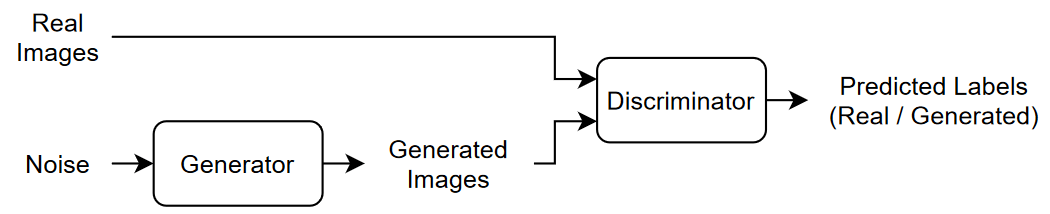
\includegraphics[width=1\linewidth]{images/TrainGenerativeAdversarialNetworkGANExample_01.png}
\end{center}
   \caption{\footnotesize This figure shows how GAN works. The image is downloaded from \href{https://de.mathworks.com/help/deeplearning/ug/train-generative-adversarial-network.html}{https://de.mathworks.com/help/deeplearning/ug/train-generative-adversarial-network.html}}
\end{figure}

By adversarial, as shown in Figure 1, we mean that the generative network and the discriminative network confront each other. The generative network tries to generate as realistic a sample as possible, while the discriminative network discriminates whether the sample is a real or generated fake sample.

Let's look back to the generative model and take the image generation model (see Figure 1.) as an example. Suppose we have an image generation model (generator) whose goal is to generate a real image. At the same time, we have an image discriminator model whose goal is to be able to correctly discriminate whether an image is generated or real. Then if we map the scenario to a game between the image generation model and the discriminator model, it becomes the following pattern: 
\begin{itemize}
    \item[1.] The generation model generates some images.
    \item[2.] The discriminator model learns to distinguish the generated images from the real ones.
    \item[3.] The generation model improves itself according to the discriminator model and generates new images.
    \item[4.] The discriminator model gets improved to learn to distinguish the generated images better.
\end{itemize}
So that is the way how two models compete adversely and improve themselves repeatedly. 

In conclusion, GAN tries to create a distribution that can match the original data distribution as shown in Figure 2.
\begin{figure}[htpb]
\begin{center}
   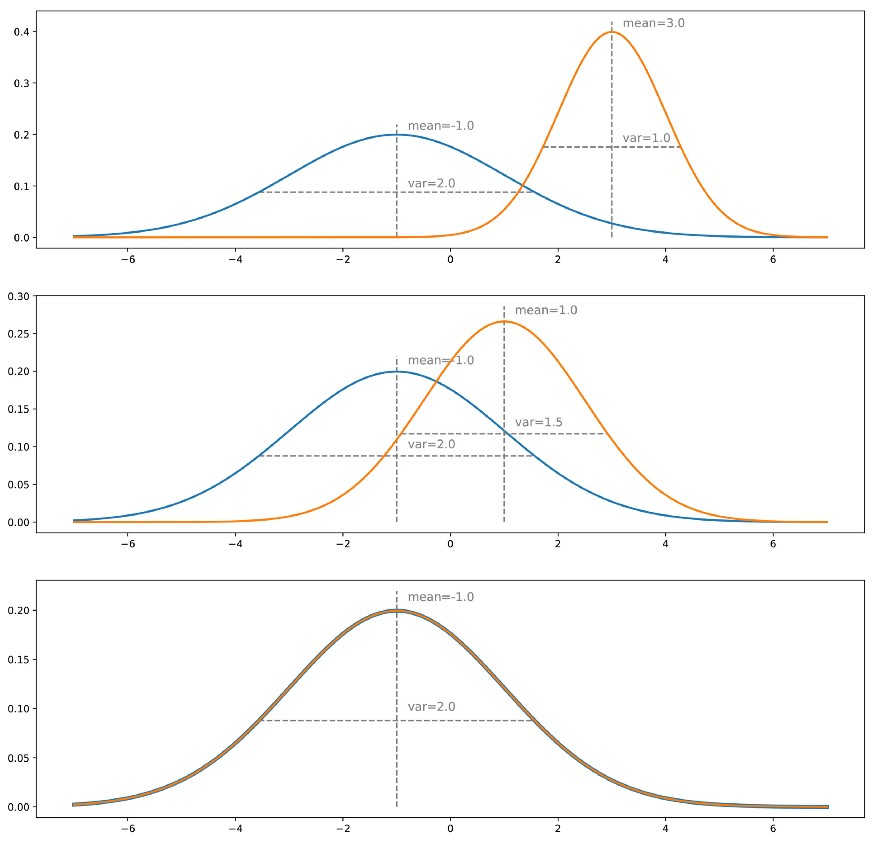
\includegraphics[width=1\linewidth, height=1.5\linewidth]{images/1_3XAUCz6o2DZlGHVsovvRIQ.jpeg}
\end{center}
   \caption{\footnotesize This figure shows how the distribution tries to match the data distribution. The image is downloaded from \href{https://towardsdatascience.com/understanding-generative-adversarial-networks-gans-cd6e4651a29}{https://towardsdatascience.com/understanding-generative-adversarial-networks-gans-cd6e4651a29}}
\end{figure}

Additionally, if we would like to generate new things, in this example: new images, we can receive noise as input and pass it into generative model (generator) using forward propagation to get new images. 

\section{Adversarial nets}
At first, we take a look in to the generator network. The objective of it is to distinguish real samples denoted by $x \sim p_{data}$ from fake samples denoted by $\Tilde{x} \sim p_g(x)$.  We can define a multilayer perceptron $D(x;\theta_d)$ which represents the probability that $x$ is from the data distribution or generated by generator, where $\theta_d$ is corresponding parameters of the discriminator network. Compared to generator, the goal of discriminator is: 
\begin{align*}
    D(\Tilde{x}) = 0 \ \ and \ \  D(x) = 1
\end{align*}
And the goal above can be reformulated by the following equation: 
\begin{align*}
    &\max\limits_{D}\big(D(x) + (1-D(\Tilde{x}))\big)\\
    \Longleftrightarrow &\max\limits_{D}\big(\log{D(x)} + \log{(1-D(G(x))}\big)
\end{align*} 
Secondly, the generator network is eager to approximate the real data distribution $p_{data}$ with the fake distribution $p_g(x)$. As talked about in selection 1.2., it receives normally Gaussian noise $z \sim p_z(z)$ as input and outputs the fake sample $\Tilde{x} = G(z)$, where $p_z(z)$ is defined as a prior on input noise variables and represents a mapping to data space as $G(z;\theta_g)$. The goal of it is stated as follows: 
\begin{align*}
    D(G(z)) = D(\Tilde{x}) = 1 
    &\Longleftrightarrow \max\limits_G\log{D(\Tilde{x})} \\
    &\Longleftrightarrow \min\limits_G\log{\big(1 - D(G(x))\big)}
\end{align*}

\begin{figure}[htpb]
\begin{center}
   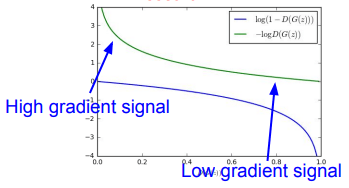
\includegraphics[scale=1]{images/1-3.png}
\end{center}
   \caption{\footnotesize This figure shows gradients of two objective functions. The image is downloaded from \href{https://projectsflix.com/machine-learning/deeplearning/types-of-gan-evaluation-metrics-of-gan/}{https://projectsflix.com/machine-learning/deeplearning/types-of-gan-evaluation-metrics-of-gan/}}
\end{figure}
Observe that we instead of minimizing likelihood of discriminator being correct, now
maximize likelihood of discriminator being wrong.
The reason is that in practice optimizing the generator objective function does not work well, because when the generated sample is likely to be classified as fake at the beginning, the model then would like to learn from the gradients. 

However, the gradients turn out to be relatively flat as shown in Figure 3. This makes it difficult for the model to learn from the gradient. Provided that we maximize the objective function, it will work much better.

Finally, we conclude that $G$ and $D$ play a two-player minimax game and can obtain the final objective function $V(G, D)$:
\begin{align*}
    &\min\limits_G\max\limits_DV(G, D)\\ &= \mathbb{E}_{x \sim p_{data}(x)}[\log{D(x)}] + \mathbb{E}_{z \sim p_z(z)}[\log{\big(1 - D(G(z))\big)}]
\end{align*}


\section{GAN Training}
\begin{algorithm}[!h]  
\caption{Minibatch stochastic gradient descent\cite{ketkar2017stochastic} training of GAN, where $t$ is number of iterations step and $k$ the number of steps to apply to the discriminator. }  \begin{algorithmic}[1]%一行一个标行号    
\FOR{$t \in \{0, .., T\}$}
    \FOR{$k$ steps}
        \STATE{Sample minibatches $x_1, ..., x_m \sim p_{data}$ and $z_1, ..., z_m \sim p_z(z)$}
        \STATE{Feed discriminator real samples $x$ and fake samples $G(z)$ for $z \sim p_z(z)$}
        \STATE{Back propagation loss gradient into $D$, update parameters:
            \begin{align*}
                &\theta_D \xleftarrow{} \theta_D + \\ &\nabla_{\theta_D} \frac{1}{m} \sum_{i=1}^m(\log{D(x_i)} + \log{(1-D(G(x_i)))})
            \end{align*}
        }
    \ENDFOR
    \STATE{Pass fake samples $G(z)$ to discriminator}
    \STATE{Back propagation loss gradient into $G$ and update parameters:
        \begin{align*}
                \theta_G \xleftarrow{} \theta_G + \nabla_{\theta_G} \frac{1}{m} \sum_{i=1}^m\big(\log{(1-D(G(x_i)))}\big)
            \end{align*}
    }
\ENDFOR
%\RETURN{} $\theta_D$, $\theta_G$
\end{algorithmic}
\end{algorithm}

In the first step, we will train the discriminator. For discriminator, in fact, it can be considered as a binary classification problem and $V(G,D)$ is then the cross entropy loss. The aim of training $D$ is to let $V(G,D)$ be as large as possible: $D(x)$ close to one and $D(G(z))$ close to zero, while generator $G$ does it oppositely, where one stands for real and zero for fake. $D$ is involved in both terms of the equation defined in Section 2:
\begin{align*}
    \max\limits_D\mathbb{E}_{x \sim p_{data}(x)}[\log{D(x)}] + \mathbb{E}_{z \sim p_z{z}}[\log{\big(1 - D(G(z))\big)}]
\end{align*}
\begin{itemize}
    \item For $\log(D(x))$: if true data is misclassified, then it leads $\log(D(x)) \ll 0$ and it is expected to be negative infinity.
    \item For $\log(1-D(G(z)))$: if generated data is as true data classified, the output trends to negative infinite as well.  
\end{itemize}

In the second step, we will train the generator. The value of $V(G, D)$ is expected to be as small as possible, so that discriminator can not distinguish between true and false data. Since the first term of $V(G, D)$ does not contain $G$: 
\begin{align*}
    \min\limits_G\mathbb{E}_{z \sim p_z{z}}[\log{\big(1 - D(G(z))\big)}]
\end{align*}
$G$ should behaves that $D(G(z))$ is close to one.  In other word, discriminator judge the generated data as true.

\section{Correctness of the training algorithm}
We assume in this case that enough capacity and training time is given. There are things needed to be proven:
\begin{itemize}
    \item $V(G, D)$ has a global optimum: $p_g = p_{data}$.
    \item The global optimum will converge during the training time.
\end{itemize}
Before proving them, let's introduce one significant concept.
\begin{definition}
The Kullback-Leibler (KL) divergence is a measure in statistics that quantifies how
close a probability distribution $p = p\{i\}$ is to a model distribution $q = \{q_i\}$:\cite{shlens2014notes}
\begin{align*}
    D_{KL}(p||q) = \sum_ip_i \cdot \log(\frac{p_i}{q_i}) 
\end{align*}
\end{definition}
Firstly, as in the training process, we will fix the generator to get the optimal discriminator.
\begin{proposition}
For fixed $G$, the optimal discriminator for any given generator $G$ is: \cite{goodfellow2014generative}
\begin{align*}
    D_G^*(x) = \frac{p_{data}(x)}{p_{data}(x) + p_g(x)}
\end{align*}
\end{proposition}

\begin{proof}
As reminder, the objective function is: 
\begin{align*}
    V(G, D) = \mathbb{E}_{x \sim p_{data}(x)}[\log{D(x)}] + \mathbb{E}_{z \sim p_z(z)}[\log{\big(1 - D(G(z))\big)}]
\end{align*}
Since $V(G,D)$ is continuous, we can rewrite it as follows:
\begin{align*}
    V(G,D)=\int_xp_{data}(x)\log{\big(D(x)\big)}dx+\int_zp_z(z)\log{\big(1-D(G(z))\big)}dz
\end{align*}
Further more, we can substitute $x$ with $G(z)$.
\begin{align}
    &x = G(z) \Longrightarrow z = G^{-1}(x)\\
    & dz = (G^{-1})^{'}(x)dx
\end{align}
And with the above equations, we are able to reformulate the objective function as:
\begin{align*}
    &V(G,D)=\int_xp_{data}(x)\log{\big(D(x)\big)}dx+\\&\int_xp_z(G^{-1}(x))\log{(1-D(x))}((G^{-1})^{'})(x)dx \\
    &=\int_xp_{data}(x)\log{\big(D(x)\big)}dx+\int_xp_g(x)\log{(1-D(x))}dx\\
    &= \int_xp_{data}(x)\log{\big(D(x)\big)}+p_g(x)\log{(1-D(x))}dx
\end{align*}
Then we should optimize $D$ such that $V(G,D)$ can reach the maximum.
\begin{align*}
    &\max_DV(G,D)\\ &= \max_D\int_xp_{data}(x)\log{\big(D(x)\big)}+p_g(x)\log{(1-D(x))}dx\\
    &\Longrightarrow\frac{\partial}{\partial{D(x)}}(p_{data}(x)\log{\big(D(x)\big)}+p_g(x)\log{(1-D(x))}) = 0\\
    &\Longrightarrow \frac{p_{data}(x)}{D(x)} - \frac{p_g(x)}{1-D(x)} = 0\\
    &\Longrightarrow D(x) = \frac{p_{data}(x)}{p_{data}(x)+p_g(x)}
\end{align*}
\end{proof}

\begin{theorem}
The global minimum of the virtual training criterion $C(G)$ is achieved if and only if $p_g = p_{data}$. At that point, $C(G)$ achieves the value $-\log{4}$.\cite{goodfellow2014generative}
\end{theorem}

\begin{proof}
From Proposition 4.1., we confirm that the optimal solution for discriminator is $D_{G(x)}^*$. Under this circumstance, the optimal solution for generator is that the generated distribution should be as similar as the real data distribution: $p_{data}(x)=p_g(x)$, which implies that  $D_{G(x)}^*$ is equal $\frac{1}{2}$. So in the next step, we should optimize $G$:
\begin{align*}
    &C(G)=\max_DV(G, D)\\
    &=\max_D\int_xp_{data}(x)\log{D(x)} + p_g(x)\log{(1-D(x))}dx
\end{align*}
Since, we know that the optimal solution of $D$ is $ D_G^*(x) = \frac{p_{data}(x)}{p_{data}(x) + p_g(x)}$, we can plug this into the above equation and max is then no more needed:
\begin{align*}
    &C(G)=\int_xp_{data}(x)\log{(D_G^*(x))})+p_g(x)\log{(1-D_G^*(x))}dx    \\
    &\Longrightarrow\int_xp_{data}(x)\log{(\frac{p_{data}(x)}{p_{data}(x)+p_g(x)}})\\
    &+p_g(x)\log{(\frac{p_{g}(x)}{p_{data}(x)+p_g(x)})}dx\\
    &\Longrightarrow\int_xp_{data}(x)\log{(\frac{p_{data}(x)}{\frac{p_{data}(x)+p_g(x)}{2}}})\\
    &+p_g(x)\log{(\frac{p_{g}(x)}{\frac{p_{data}(x)+p_g(x)}{2}})}dx-2\log{2}\\
    &=KL[p_{data}||\frac{p_{data}(x)+p_g(x)}{2}] + KL[p_g(x)||\frac{p_{data}(x)+p_g(x)}{2}]-\log{4}
\end{align*}
Since KL-Divergence is non-negative:
\begin{align*}
    \min_GC(G) = 0 + 0 - \log(4) = -\log(4)
\end{align*}
\end{proof}

\section{Implementation and experiment}

\subsection{Improvement especially for images}

\section{Disadvantage of GAN}

\subsection{Further work}

\section{Conclusion}

{\small
\bibliographystyle{ieee}
\bibliography{egbib}
}

\end{document}
